\documentclass[journal]{IEEEtran}
\usepackage{blindtext}
\usepackage{graphicx}
\usepackage[version=3]{mhchem} % Package for chemical equation typesetting
\usepackage{siunitx} % Provides the \SI{}{} and \si{} command for typesetting SI units
%\usepackage{natbib} % Required to change bibliography style to APA
\usepackage{amsmath} % Required for some math elements 

% Paquetes a usar
%\usepackage[spanish]{babel}   %%para Colocar el Español
\usepackage[utf8]{inputenc} %%para usar tildes adecuadamente
\usepackage{amssymb}          % Símbolos
\usepackage{hyperref}         % Vinculos 
\usepackage{graphics}         % Subfiguras
\usepackage{pdfpages}         % incluir PDF
\usepackage[tight,footnotesize]{subfigure}
\usepackage[spanish]{babel}   %%para Colocar el Español
\usepackage{pgfplots}

\usepackage{filecontents,lipsum}
\usepackage[noadjust]{cite}
\begin{filecontents*}{references.bib}
@article{Khoe:1994:CML:2288694.2294265,
    author = {Khoe, G. -D.},
    title = {Coherent multicarrier lightwave technology for flexible capacity networks},
    journal = {Comm. Mag.},
    issue_date = {March 1994},
    volume = {32},
    number = {3},
    month = mar,
    year = {1994},
    issn = {0163-6804},
    pages = {22--33},
    numpages = {12},
    url = {http://dx.doi.org/10.1109/35.267438},
    doi = {10.1109/35.267438},
    acmid = {2294265},
    publisher = {IEEE Press},
    address = {Piscataway, NJ, USA},
}

@article{cegomez,
title = "Responses of the tropical gorgonian coral Eunicea fusca to ocean acidification conditions",
keywords = "Calcein, Carbonate saturation state, Caribbean, Ocean acidification, Tropical gorgonian",
author = "Gómez, {C. E.} and Paul, {V. J.} and R. Ritson-Williams and N. Muehllehner and C. Langdon and Sánchez, {J. A.}",
year = "2015",
month = "6",
doi = "10.1007/s00338-014-1241-3",
volume = "34",
pages = "451--460",
journal = "Coral Reefs",
issn = "0722-4028",
number = "2",
}

@INPROCEEDINGS{estrellas,
author={A. Mendes and M. Hoeberechts and A. B. Albu},
booktitle={Applications and Computer Vision Workshops (WACVW), 2015 IEEE Winter},
title={Evolutionary Computational Methods for Optimizing the Classification of Sea Stars in Underwater Images},
year={2015},
pages={44-50},
keywords={evolutionary computation;geophysical image processing;image classification;image sampling;oceanographic techniques;video signal processing;automated processing method;automatic classification;classification process;evolutionary computational method;human analyst;imagery;marine organism;sampling method;sea star classification;underwater images;video;Feature extraction;Genetic algorithms;Image segmentation;Marine animals;Optimization;Shape;Support vector machine classification},
doi={10.1109/WACVW.2015.9},
month={Jan},}

@INPROCEEDINGS{exprobots,
author={A. Maldonado-Ramírez and L. A. Torres-Méndez},
booktitle={OCEANS 2015 - Genova},
title={Autonomous robotic exploration of coral reefs using a visual attention-driven strategy for detecting and tracking regions of interest},
year={2015},
pages={1-5},
keywords={autonomous underwater vehicles;object detection;object tracking;robot vision;video signal processing;coral reefs;regions of interest detection;regions of interest tracking;superpixel descriptors;underwater environments;underwater scenes;video-observations;visual attention-driven strategy;visual-based autonomous robotic exploration;Collision avoidance;Computational modeling;Image color analysis;Navigation;Robot kinematics;Visualization},
doi={10.1109/OCEANS-Genova.2015.7271757},
month={May},}

@inproceedings{slope,
author={M. R. Algodon and A. Hilomen and M. Soriano},
booktitle={OCEANS 2015 - MTS/IEEE Washington},
title={Estimating coral reef slope or camera pitch from video},
year={2015},
pages={1-5},
keywords={cameras;image motion analysis;video signal processing;benthos monitoring setup;camera pitch;camera rotation angle distorting effect elimination;coral colony area estimation;coral reef slope estimation;image feature movement;reef slope distorting effect elimination;tracks;video image improvement;Cameras;Correlation;Estimation;Feature extraction;Mathematical model;Sea measurements;Tracking;Camera Rotation;Coral Assessment;Coral Reef Slope},
month={Oct},}

@INPROCEEDINGS{pequenosinforma,
author={O. Beijbom and P. J. Edmunds and D. I. Kline and B. G. Mitchell and D. Kriegman},
booktitle={Computer Vision and Pattern Recognition (CVPR), 2012 IEEE Conference on},
title={Automated annotation of coral reef survey images},
year={2012},
pages={1170-1177},
keywords={cameras;ecology;geophysical image processing;image colour analysis;image texture;oceanographic techniques;rocks;sand;Moorea Labeled Corals;algae;automatic acquisition systems;class variation;color descriptors;computer vision community;coral reef coverage estimation;coral reef survey images;digital cameras;ecological data;expert annotations;image libraries;image quality;manual image analysis;multiyear dataset;performance benchmarking;quantitative analysis;reef surface;reliable automated coral reef image annotation;rock;sand;texture descriptors;valuable scientific data;viewpoints;Algae;Benchmark testing;Computer vision;Histograms;Image color analysis;Shape;Vectors},
doi={10.1109/CVPR.2012.6247798},
ISSN={1063-6919},
month={June},}

@INPROCEEDINGS{autopistas,
author={A. K. Tripathi and S. Swarup},
booktitle={Advance Computing Conference (IACC), 2013 IEEE 3rd International},
title={Shape and color features based airport runway detection},
year={2013},
pages={836-841},
keywords={feature extraction;filtering theory;image colour analysis;image denoising;image segmentation;object detection;Frangi filter;airport runway detection;anisotropic diffusion;chroma based feature;color feature;commercial application;defence application;false runway candidate;noise immunity;qualitative analysis;quantitative analysis;runway segmentation;shape feature;Airports;Algorithm design and analysis;Detection algorithms;Image color analysis;Image segmentation;Roads;Shape;Frangi filter;Runway;anisotropic diffusion;chroma features and tubular structure},
doi={10.1109/IAdCC.2013.6514335},
month={Feb},}

@INPROCEEDINGS{flujo,
author={E. Türetken and C. Becker and P. Glowacki and F. Benmansour and P. Fua},
booktitle={2013 IEEE International Conference on Computer Vision},
title={Detecting Irregular Curvilinear Structures in Gray Scale and Color Imagery Using Multi-directional Oriented Flux},
year={2013},
pages={1553-1560},
keywords={image colour analysis;object detection;optimisation;biological imagery;color datasets;color imagery;complex optimization problem;gray scale datasets;gray scale imagery;image gradient flux maximization;irregular curvilinear structure detection;multidirectional oriented flux;noisy image stacks;radii;Biomedical imaging;Biomedical measurement;Color;Eigenvalues and eigenfunctions;Image color analysis;Vectors;Curvilinear networks;curvilinear structures;image gradient flux;multi-directional oriented flux;optimally oriented flux;segmentation;tubular structures;tubularity measure},
doi={10.1109/ICCV.2013.196},
ISSN={1550-5499},
month={Dec},}

@ARTICLE{espina,
author={B. De Leener and J. Cohen-Adad and S. Kadoury},
journal={IEEE Transactions on Medical Imaging},
title={Automatic Segmentation of the Spinal Cord and Spinal Canal Coupled With Vertebral Labeling},
year={2015},
volume={34},
number={8},
pages={1705-1718},
keywords={biomedical MRI;bone;diseases;image segmentation;image sequences;injuries;medical image processing;neurophysiology;Dice coefficients;MRI contrast;PropSeg method;SC injury;T1-weighted sequences;T2*-weighted sequences;T2-weighted sequences;automatic intervertebral disk identification method;automatic segmentation;bias-free measurement;clinician diagnosis;clinician prognosis;generic coordinate system;intersubject comparison;intrasubject comparison;multiresolution propagation;neurodegenerative diseases;spinal canal;spinal cord atrophy;traumatic diseases;tubular deformable models;vertebral labeling;vertebral level identification method;vertebral-based normalization;Deformable models;Image segmentation;Irrigation;Mathematical model;Measurement;Spinal cord;Transforms;Automatic segmentation;CSF;MRI;deformable model;spinal canal;spinal cord;vertebral labeling},
doi={10.1109/TMI.2015.2437192},
ISSN={0278-0062},
month={Aug},}

@INPROCEEDINGS{opti,
author={A. Jezierska and O. Miraucourt and H. Talbot and S. Salmon and N. Passat},
booktitle={2014 IEEE International Conference on Image Processing (ICIP)},
title={A non-local chan-vese model for sparse, tubular object segmentation},
year={2014},
pages={907-911},
keywords={image segmentation;object detection;optimisation;Chan-Vese framework;continuous optimization scheme;nonlocal fitting term;object sparsity;piecewise-constant model;sparse object segmentation;tubular object segmentation;Biomedical imaging;Context;Image segmentation;Noise;Optimization;Retina;Three-dimensional displays;Variational image segmentation;angiographic imaging;nonlocal data fidelity;tubular structures},
doi={10.1109/ICIP.2014.7025182},
ISSN={1522-4880},
month={Oct},}

@article{stokes_automated_2009,
	title = {Automated processing of coral reef benthic images: {Coral} reef benthic imaging},
	volume = {7},
	issn = {15415856},
	shorttitle = {Automated processing of coral reef benthic images},
	url = {http://doi.wiley.com/10.4319/lom.2009.7.157},
	doi = {10.4319/lom.2009.7.157},
	language = {en},
	number = {2},
	urldate = {2016-04-26TZ},
	journal = {Limnology and Oceanography: Methods},
	author = {Stokes, M. Dale and Deane, Grant B.},
	month = feb,
	year = {2009},
	pages = {157--168}
}

@article{schindelin_fiji:_2012,
	title = {Fiji: an open-source platform for biological-image analysis},
	volume = {9},
	issn = {1548-7091, 1548-7105},
	shorttitle = {Fiji},
	url = {http://www.nature.com/doifinder/10.1038/nmeth.2019},
	doi = {10.1038/nmeth.2019},
	number = {7},
	urldate = {2016-04-26TZ},
	journal = {Nature Methods},
	author = {Schindelin, Johannes and Arganda-Carreras, Ignacio and Frise, Erwin and Kaynig, Verena and Longair, Mark and Pietzsch, Tobias and Preibisch, Stephan and Rueden, Curtis and Saalfeld, Stephan and Schmid, Benjamin and Tinevez, Jean-Yves and White, Daniel James and Hartenstein, Volker and Eliceiri, Kevin and Tomancak, Pavel and Cardona, Albert},
	month = jun,
	year = {2012},
	pages = {676--682}
}

@inproceedings{gulshan_geodesic_2010,
	title = {Geodesic star convexity for interactive image segmentation},
	isbn = {978-1-4244-6984-0},
	url = {http://ieeexplore.ieee.org/lpdocs/epic03/wrapper.htm?arnumber=5540073},
	doi = {10.1109/CVPR.2010.5540073},
	urldate = {2016-04-26TZ},
	publisher = {IEEE},
	author = {Gulshan, Varun and Rother, Carsten and Criminisi, Antonio and Blake, Andrew and Zisserman, Andrew},
	month = jun,
	year = {2010},
	pages = {3129--3136}
}

@article{hoegh-guldberg_coral_2007,
	title = {Coral {Reefs} {Under} {Rapid} {Climate} {Change} and {Ocean} {Acidification}},
	volume = {318},
	issn = {0036-8075, 1095-9203},
	url = {http://www.sciencemag.org/cgi/doi/10.1126/science.1152509},
	doi = {10.1126/science.1152509},
	language = {en},
	number = {5857},
	urldate = {2016-04-26TZ},
	journal = {Science},
	author = {Hoegh-Guldberg, O. and Mumby, P. J. and Hooten, A. J. and Steneck, R. S. and Greenfield, P. and Gomez, E. and Harvell, C. D. and Sale, P. F. and Edwards, A. J. and Caldeira, K. and Knowlton, N. and Eakin, C. M. and Iglesias-Prieto, R. and Muthiga, N. and Bradbury, R. H. and Dubi, A. and Hatziolos, M. E.},
	month = dec,
	year = {2007},
	pages = {1737--1742}
}

@article{treibitz_wide_2015,
	title = {Wide {Field}-of-{View} {Fluorescence} {Imaging} of {Coral} {Reefs}},
	volume = {5},
	issn = {2045-2322},
	url = {http://www.nature.com/articles/srep07694},
	doi = {10.1038/srep07694},
	urldate = {2016-04-26TZ},
	journal = {Scientific Reports},
	author = {Treibitz, Tali and Neal, Benjamin P. and Kline, David I. and Beijbom, Oscar and Roberts, Paul L. D. and Mitchell, B. Greg and Kriegman, David},
	month = jan,
	year = {2015},
	pages = {7694}
}

@article{neal_methods_2015,
	title = {Methods and measurement variance for field estimations of coral colony planar area using underwater photographs and semi-automated image segmentation},
	volume = {187},
	issn = {0167-6369, 1573-2959},
	url = {http://link.springer.com/10.1007/s10661-015-4690-4},
	doi = {10.1007/s10661-015-4690-4},
	language = {en},
	number = {8},
	urldate = {2016-04-26TZ},
	journal = {Environmental Monitoring and Assessment},
	author = {Neal, Benjamin P. and Lin, Tsung-Han and Winter, Rivah N. and Treibitz, Tali and Beijbom, Oscar and Kriegman, David and Kline, David I. and Greg Mitchell, B.},
	month = aug,
	year = {2015}
}

@article{schneider_nih_2012,
	title = {{NIH} {Image} to {ImageJ}: 25 years of image analysis},
	volume = {9},
	issn = {1548-7105},
	shorttitle = {{NIH} {Image} to {ImageJ}},
	abstract = {For the past 25 years NIH Image and ImageJ software have been pioneers as open tools for the analysis of scientific images. We discuss the origins, challenges and solutions of these two programs, and how their history can serve to advise and inform other software projects.},
	language = {eng},
	number = {7},
	journal = {Nature Methods},
	author = {Schneider, Caroline A. and Rasband, Wayne S. and Eliceiri, Kevin W.},
	month = jul,
	year = {2012},
	pmid = {22930834},
	keywords = {Computational Biology, History, 20th Century, History, 21st Century, Image Processing, Computer-Assisted, National Institutes of Health (U.S.), Software, United States},
	pages = {671--675}
}

@article{acidificacion,
 author = "Hoegh-Guldberg, O. and P. J. Mumby and A. J. Hooten and R. S. Steneck and P. Greenfield and E. Gomez and C. D. Harvell and P. F. Sale and A. J. Edwards and K. Caldeira",
 title = "Coral reefs under rapid climate change and ocean acidification",
 journal = "Science",
 volume = "318",
 number = "742",
 pages = "1",
 year = 2007
}

@article{scikit-image,
 title = {scikit-image: image processing in {P}ython},
 author = {van der Walt, {S}t\'efan and {S}ch\"onberger, {J}ohannes {L}. and
           {Nunez-Iglesias}, {J}uan and {B}oulogne, {F}ran\c{c}ois and {W}arner,
           {J}oshua {D}. and {Y}ager, {N}eil and {G}ouillart, {E}mmanuelle and
           {Y}u, {T}ony and the scikit-image contributors},
 year = {2014},
 month = {6},
 keywords = {Image processing, Reproducible research, Education,
             Visualization, Open source, Python, Scientific programming},
 volume = {2},
 pages = {e453},
 journal = {PeerJ},
 issn = {2167-8359},
 url = {http://dx.doi.org/10.7717/peerj.453},
 doi = {10.7717/peerj.453}
}

\end{filecontents*}

\renewcommand{\contentsname}{Tabla de contenido}
\renewcommand{\partname}{Parte}
\renewcommand{\appendixname}{Apéndice}
%\renewcommand{\bibname}{Referencias}
\renewcommand{\figurename}{Figura}
\renewcommand{\listfigurename}{Índice de figuras}
\renewcommand{\tablename}{Tabla}
\renewcommand{\listtablename}{Índice de tablas}

\ifCLASSINFOpdf
 
\else

\fi

\hyphenation{op-tical net-works semi-conduc-tor}

\begin{document}

\title{Automatización de detección de crecimiento de estructuras coralinas}

\author{Sergio Daniel Hernández Charpak,~\IEEEmembership{}
        José Francisco Molano Pulido~\IEEEmembership{}% <-this % stops a space
\thanks{}% <-this % stops a space
\thanks{}% <-this % stops a space
\thanks{}}

% The paper headers
\markboth{Imágenes y Visión, primer semestre 2016}%
{Shell \MakeLowercase{\textit{et al.}}: Bare Demo of IEEEtran.cls for Journals}

\maketitle


\begin{abstract}
%\boldmath
El crecimiento del área del coral está influenciado por el nivel de acidez del mar. 
Se tomaron en laboratorio varias muestras del coral. Se exponen estas muestras a
varios niveles de acidez. Medir el área del coral a partir de fotografías ha sido un reto en
este tema. Este reto ha sido examinado en fotografías en campo más no en fotografías en
laboratorio, donde el montaje puede facilitar enormemente el análisis de las imágenes. Nosotros
en este trabajo automatizamos la segmentación de imágenes de coral tomadas bajo un montaje
definido en laboratorio. Obtuvimos resultados satisfactorios y prometedores. Finalmente,
discutimos varios factores pueden influenciar nuestros resultados.
\end{abstract}
%TODO ESCRIBIR EL NOMBRE DEL CORAL EN EL ABSTRACT
%\begin{IEEEkeywords}
%IEEEtran, journal, \LaTeX, paper, template.
%\end{IEEEkeywords}

\IEEEpeerreviewmaketitle

\section{Introducción}

\begin{par}
En la actualidad, uno de los fenómenos que más preocupan a la comunidad científica en relación a los ecosistemas marinos corresponde a la acidificación del océano. Este fenómeno, ocasionado por un incremento de las concentraciones de dióxido de carbono atmosférico, es una amenaza preocupante para los sistemas coralinos. Esto se debe a que la acidificación del océano afecta directamente al proceso acreción de carbonato, el cual corresponde al mecanismo de crecimiento de dichos organismos \cite{acidificacion}. Por este motivo, el análisis del crecimiento en estructuras coralinas resulta de gran importancia en el campo de la biología marina. Hoy en día, éste corresponde a uno de los principales métodos para medir el impacto de la acidificación y del incremento de los niveles de dióxido de carbono en la atmósfera.
\end{par}
\begin{par}
Actualmente, el estudio del crecimiento de estos organismos se ve fundamentado en el análisis de imágenes ópticas, que son adquiridas tanto en el hábitat natural como en entornos de laboratorio. En ambos casos, el objetivo principal de dichas tomas corresponde a realizar una medida del crecimiento de los corales sin recurrir a métodos invasivos. Finalmente, se efectúa el análisis de las imágenes obtenidas al estimar parámetros como el área o la longitud de los organismos mediante diversos métodos. En particular, es posible observar en la literatura que varios estudios hacen uso de métodos computacionales con la finalidad de automatizar el proceso de definición de parámetros, esto resulta particularmente provechoso teniendo en cuenta que este tipo de análisis requiere del procesamiento de un número considerable de imágenes. Sin embargo, en muchos casos, los investigadores se ven obligados a emplear métodos manuales, principalmente porque no disponen de herramientas especializadas para obtener los parámetros de interés en cada caso particular.
\end{par}
\begin{par}
En particular, se tiene que el grupo de investigación Biommar de la Universidad de los Andes no dispone de herramientas especializadas para el análisis de imágenes de corales, por este motivo dicho análisis es realizado de forma manual. El objetivo del presente trabajo consistió en dar soporte a este grupo desarrollando un producto de software para determinar los parámetros de interés en el caso específico de muestras de laboratorio. El método desarrollado permite la obtención del área de los corales a través de una serie de imágenes ingresada por parámetro. El algoritmo implementado hace uso de técnicas ligeras de procesamiento para obtener las respectivas medidas y calcular la diferencia entre los componentes de la secuencia, para efectos prácticos, esto corresponde al crecimiento del coral en cuestión. El producto de software se presenta como una propuesta diferenciadora a alternativas similares debido a su carácter de código abierto. Éste puede ser modificado por medio de procesos relativamente sencillos para acoplarse a requerimientos del mismo tipo, evitando también que los grupos de investigación interesados incurran en el pago de licencias para productos comerciales.
\end{par}
\begin{par}
El presente documento realiza una breve exposición de los métodos observados en la literatura para cumplir con el mismo objetivo y con objetivos similares, posteriormente, se hace una breve presentación del método implementado. Luego, se presentan los resultados obtenidos al emplear el producto de software en imágenes de prueba con su respectiva validación y finalmente se exponen las conclusiones relacionadas con la solución propuesta y con el proceso que se llevó a cabo para la obtención de la misma.
\end{par}


\section{Estado del Arte}
En el campo de la biología marina, la evaluación de las principales características de
los organismos coralinos ha sido soportada por el análisis de imágenes. Mendes
\cite{estrellas} hace énfasis en que este método corresponde a una alternativa no
invasiva, factor que resulta importante para la conservación del medio ambiente evitando
la perturbación de los hábitats. Adicionalmente resalta el hecho de que, particularmente
en las últimas décadas, el análisis de imágenes para el estudio de los organismos marinos
se ha apoyado fundamentalmente en las técnicas computacionales. El uso de estas
herramientas permite manejar grandes volúmenes de información y obtener resultados más
precisos en aplicaciones que antes eran realizadas mediante procesos manuales. 

El trabajo realizado en la presente década, en materia de métodos computacionales para el
estudio de corales, se ha centrado principalmente en el desarrollo de técnicas de
procesamiento para imágenes adquiridas \textit{in situ}, es decir que han sido obtenidas
directamente en el hábitat de los organismos a analizar. Es por este motivo que las
investigaciones realizadas en este período se enfocan en los retos que supone la toma de
imágenes en entornos no controlados. De esta manera es posible observar propuestas
centradas en tareas como la corrección de fotografías debido a la inclinación de los
dispositivos de captura o a pendientes en el suelo marino \cite{slope}, la identificación
y caracterización de objetos en videos obtenidos mediante exploración robótica autónoma
\cite{exprobots} y la segmentación en imágenes con estructuras pequeñas sin bordes ni
formas definidas \cite{pequenosinforma}. Si bien los distintos enfoques expuestos cumplen
con el objetivo de apoyar procesos para determinar las características principales de las
organismos coralinos, éstos no son aplicables a las condiciones de laboratorio propias
del presente proyecto. 

Un enfoque más aproximado a la detección de crecimiento de corales en condiciones de
laboratorio, dada la geometría característica de las estructuras desarrolladas en este
caso, corresponde a las técnicas de segmentación de estructuras tubulares. Este también
corresponde a un campo ampliamente estudiado en la disciplina del procesamiento de
imágenes debido a su extenso margen de aplicación. En particular, se han identificado
tres categorías principales en las que se pueden clasificar los métodos de segmentación
de estructuras tubulares: métodos manuales asistidos, métodos semi-automáticos y
métodos automáticos.


\subsection{Métodos manuales asistidos}

Gran parte de los trabajos en el campo de la segmentación de imágenes biológicas
involucra una interacción del experto con un software especializado. Describimos los
métodos manuales más sofisticados que \textit{dibujar} el contorno de un objeto sobre una
imagen, alternativa que aún es presentada como viable \cite{neal_methods_2015} cuando las imágenes son de alta complejidad.

Existen numerosos métodos de segmentación para asistir interactivamente al usuario.
Nombramos uno de ellos, el método de estrellas geodésicas convexas, propuesto por Gulshan
et al., \cite{gulshan_geodesic_2010}, ya que es usado en el campo relevante a este
trabajo \cite{treibitz_wide_2015} y brinda buenos resultados.

La distribución Fiji
de ImageJ \cite{schindelin_fiji:_2012} es actualmente el software estado del arte en este
campo y lleva más de 25 años \cite{schneider_nih_2012} siendo utilizado en este a través
de sus distintas evoluciones. Sin embargo la interacción consume tiempo, dependiendo del
problema. En el trabajo
de Stokes et al \cite{stokes_automated_2009} de clasificación de especies de corales en
imágenes \textit{in situ}, el análisis de clasificación manual toma entre 15-30 min dependiendo de la
complejidad de la imagen. Trabajando con grandes conjuntos de datos el tiempo (y costo)
del experto se vuelven inviables.

%Posicion
Para imágenes complejas evitar la interacción de un experto es difícil. Sin embargo, para
imágenes simples evitar dicha interacción para poder analizar grandes cantidades de
imágenes es deseable y en este caso, es la prioridad en el marco de este proyecto.


\subsection{Métodos semi-automáticos}
%Esto quizas podria no ponerse
Automatizar los métodos de análisis de imágenes hace parte de los retos en este campo.
%Gin de lo que podría no ponerse
Se han obtenido resultados relevantes a través de métodos semi-asistidos o
semi-automáticos. 

Treibitz et al. \cite{treibitz_wide_2015}, basándose en el método de
Gulshan et al. \cite{gulshan_geodesic_2010}, desarrollan un método semi-asistido para
imágenes \textit{in situ} fluorescentes de campo amplio de corales. El usuario interactiva indica
brevemente el ruido y una región de objeto. El algoritmo segmenta los objetos dados estos
datos. El tratamiento que enseguida se le hace a los objetos es automatizado
(no-interactivo). Así, logran mostrar una correlación entre los espectros resultantes
de este tratamiento y las medidas de espectrómetro de los mismos corales. 

De la misma manera, Neal et al. \cite{neal_methods_2015}, con el objetivo de hacer medición de las varianzas de de estimaciones de campo en colonias de corales, utiliza una
segmentación de imágenes \textit{in situ} interactiva en la que se indican ruido y objetos antes de que el software identifique los contornos. El usuario tiene la posibilidad de corregir dichos contornos. El análisis que luego hace el software es independiente y efectivo.

\subsection{Métodos automáticos}
Esta categoría corresponde al conjunto de métodos más relevante para el desarrollo del
presente proyecto en la medida en que uno de los requerimientos más importantes del mismo
corresponde a la caracterización sistemática, en términos de tamaño, de los organismos
coralinos sin intervención alguna del usuario. En particular, estas técnicas hacen uso de
algoritmos basados en niveles de intensidad, colores y detección de formas con la
finalidad de identificar objetos de interés.

En primer lugar, se destaca el método propuesto por Tripathi et. al. \cite{autopistas}
para la identificación de autopistas en imágenes aéreas, el cual consta de dos etapas
principales: segmentación gruesa y refinamiento. La primera etapa hace uso de los niveles
de intensidad y la geometría presente en la imagen para realizar una selección preliminar
de un conjunto de píxeles de interés. Posteriormente, se realiza el refinamiento
respectivo para seleccionar los píxeles finales por medio de un análisis de croma y
formas. Este algoritmo resulta interesante para la identificación de estructuras
tubulares debido a la aplicación de una etapa previa de segmentación general, esto
permite que su respectiva ejecución sea más eficiente en relación a otras técnicas.

Asimismo, se destaca el uso de algoritmos basados en la curvatura. Turetken et. al.
\cite{flujo} demostraron la efectividad de emplear conceptos asociados al flujo en
estructuras tubulares para la segmentación de objetos. En particular han empleado el
flujo óptimo orientado (OOF), el flujo orientado multi-dimensional (MDOF) y el flujo
orientado antisimétrico (OFA) para la identificación de estructuras de interés,
principalmente vasos sanguíneos en imágenes médicas. Estos métodos resultan
particularmente interesantes debido a que son poco susceptibles a errores de segmentación
debido a estructuras adyacentes.

Finalmente, se destaca el caso de la segmentación basada en la identificación de figuras
geométricas. Para ilustrar este punto, se puede tomar como referencia la investigación
desarrollada por De Leener et. al. \cite{espina} quienes propusieron un método para la
identificación de vértebras en la espina dorsal, una estructura tubular, basándose en la
detección de elipses y tomando provecho de las características de simetría de la anatomía
humana. Este método se destaca entre los demás debido a que permite, además de la
segmentación de la espina dorsal, el etiquetamiento sobre las vértebras que componen
dicha estructura.\\
Estos métodos no resultan muy apropiados para el caso particular debdio a que este puede ser solventado mediante niveles de gris.

\section{Métodos}

\begin{itemize}
    \item Captura de las imágenes
\end{itemize}

\begin{par}
Definir ciertos estándares en la captura de imágenes facilita su procesamiento. Debido a que el objetivo es de calcular áreas de corales, se propuso que la captura de imágenes tuviera las siguientes características:
\begin{enumerate}
    \item un fondo que contraste con el coral,
    \item en la parte superior de la imagen, un cuadrado negro de 1 $cm^2$ que servirá de escala.
    \item el coral en su base completa en la parte inferior de la imagen.
    \item una iluminación para que haya un contraste entre base y estructura coralina.
\end{enumerate}
En el marco de este trabajo, se capturaron imágenes en diferentes
calidades. Se comprobó que para que el método funcione correctamente no
es necesaria una alta calidad de la imagen. El montaje fue realizado por 
un miembro del grupo Biommar. En la figura \ref{fg:ejemplo_foto} se puede observar una de las imágenes capturadas.
\end{par}

\begin{figure}[ht]
\begin{center}
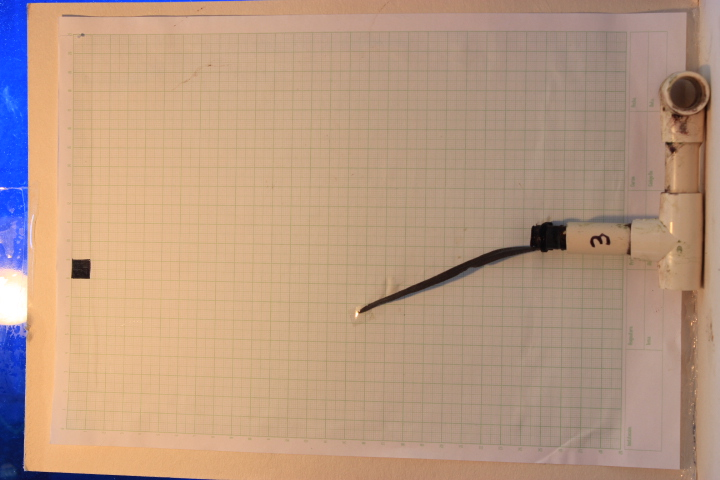
\includegraphics[width=0.37\textwidth]{fotos/Coral_3_S3} % Include the image placeholder.png
\caption{Un ejemplo del nuevo montaje de captura de imágenes}
\label{fg:ejemplo_foto}
\end{center}
\end{figure}
\FloatBarrier

\begin{itemize}
    \item Python y Scikit-image
\end{itemize}
\begin{par}
Python es uno de los lenguajes de alto nivel en el contexto actual cuyo
uso es generalizado en la comunidad científica. Como lenguaje facilita la
integración con librerías abiertas y desarrolladas por expertos. En el
marco de este trabajo se hizo uso de las librerías científicas de Python
tales como Numpy, Matplotlib, Pylab y scikit-image.\\
La librería en Python scikit-image \cite{scikit-image} es una librería reciente, mantenida, completa, para el análisis de imágenes en Python. Brinda un número extensivo de funciones y métodos para ello y su curva de aprendizaje es menor.
\end{par}


\begin{itemize}
    \item Umbralización
\end{itemize}
\begin{par}
El primer tratamiento que se decidió hacerle a las imágenes fue pasarlas
a niveles de grises para enseguida umbralizarlas para obtener imágenes
binarias. Las imágenes binarias son mucho más simples de tratar que las
imágenes a color RGB o a escala de grises. En la figura
\ref{fg:ejemplo_histograma} se puede observar el histograma de la imagen
en la figura \ref{fg:ejemplo_foto}. Es claro como este histograma es
bimodal, es decir que su histograma se puede ver como la suma de dos
funciones gausianas. Esto es una consecuencia natural de la captura de
las imágenes al tener en contraste el coral y el cuadrado de 1 $cm^2$ con
respecto al resto de la imagen. \\

La umbralización Otsu es un método que está hecho para histogramas
bimodales. El método busca el valor de gris que separe los dos modos que
minimice la varianza individual de cada uno de estos. Para optimizar el
resultado y evitar discrepancias debidas a la iluminación en la toma de
la imagen, se aplica esta umbralización de manera independiente a la
sección superior de la imagen y a la sección restante de la imagen. En
las figuras \ref{fg:square_otsu} y \ref{fg:coral_otsu} se pueden observar
los resultados con los cuales se forma la imagen umbralizada, figura
\ref{fg:umbral}, que será enseguida procesada.
\end{par}

\begin{figure}[ht]
\begin{center}
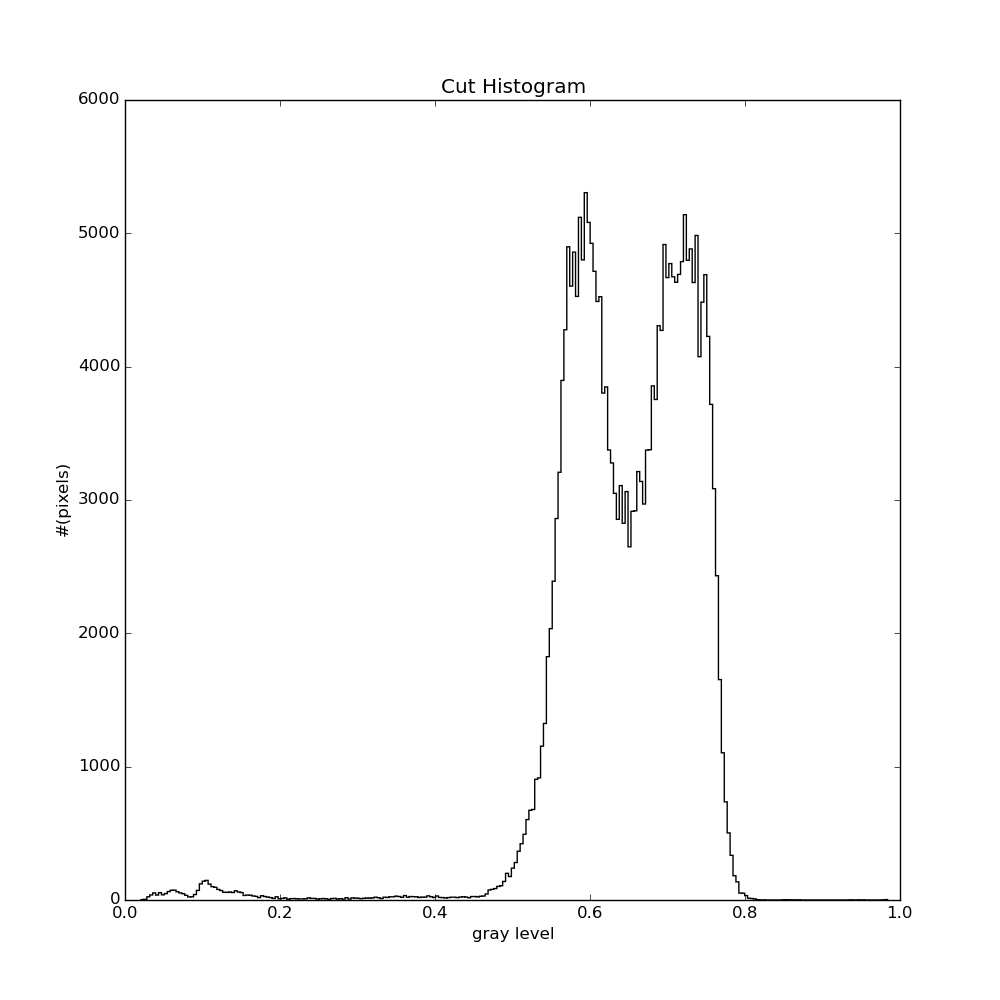
\includegraphics[width=0.37\textwidth]{resultados/Coral_3_S3_histogram} % Include the image placeholder.png
\caption{Un ejemplo del histograma de la imagen en escala de grises}
\label{fg:ejemplo_histograma}
\end{center}
\end{figure}
\FloatBarrier

\begin{figure}[ht]
\begin{center}
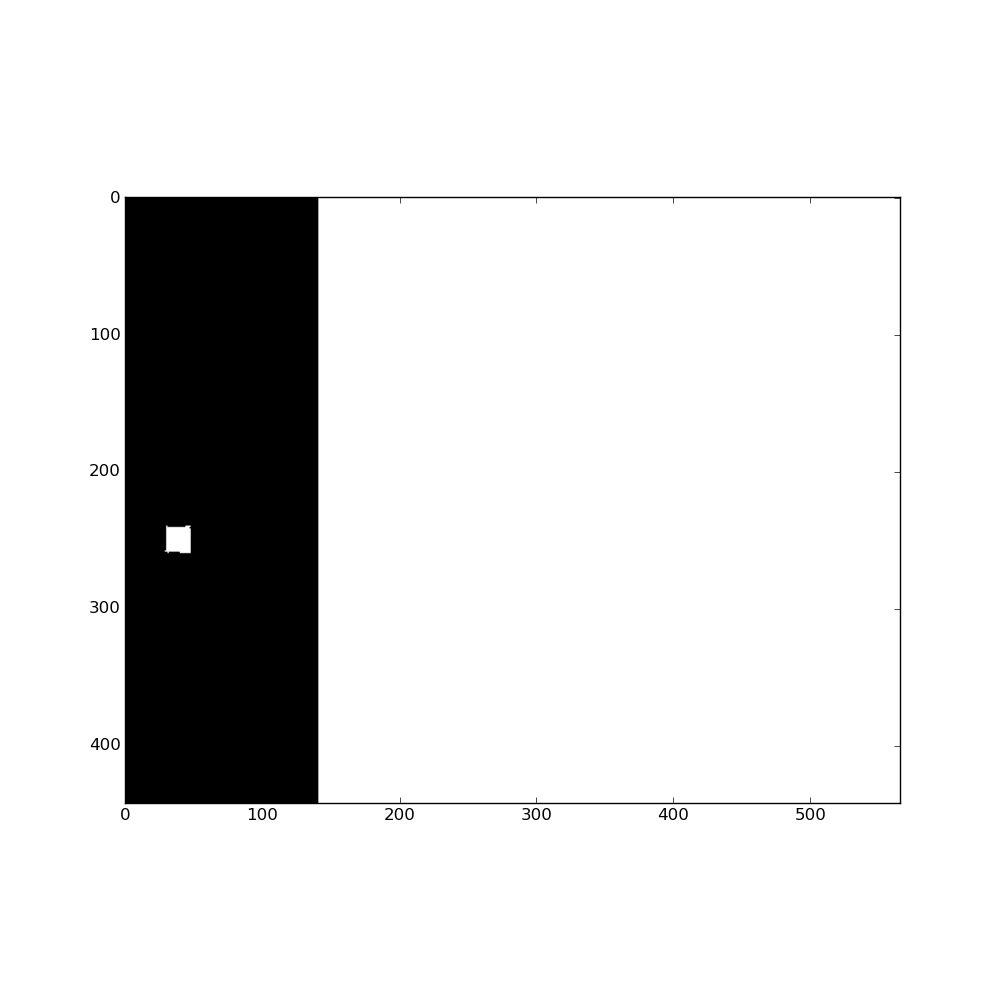
\includegraphics[width=0.37\textwidth]{resultados/Coral_3_S3_square_otsu} % Include the image placeholder.png
\caption{Umbralización Otsu sobre la sección superior de la imagen}
\label{fg:square_otsu}
\end{center}
\end{figure}
\FloatBarrier

\begin{figure}[ht]
\begin{center}
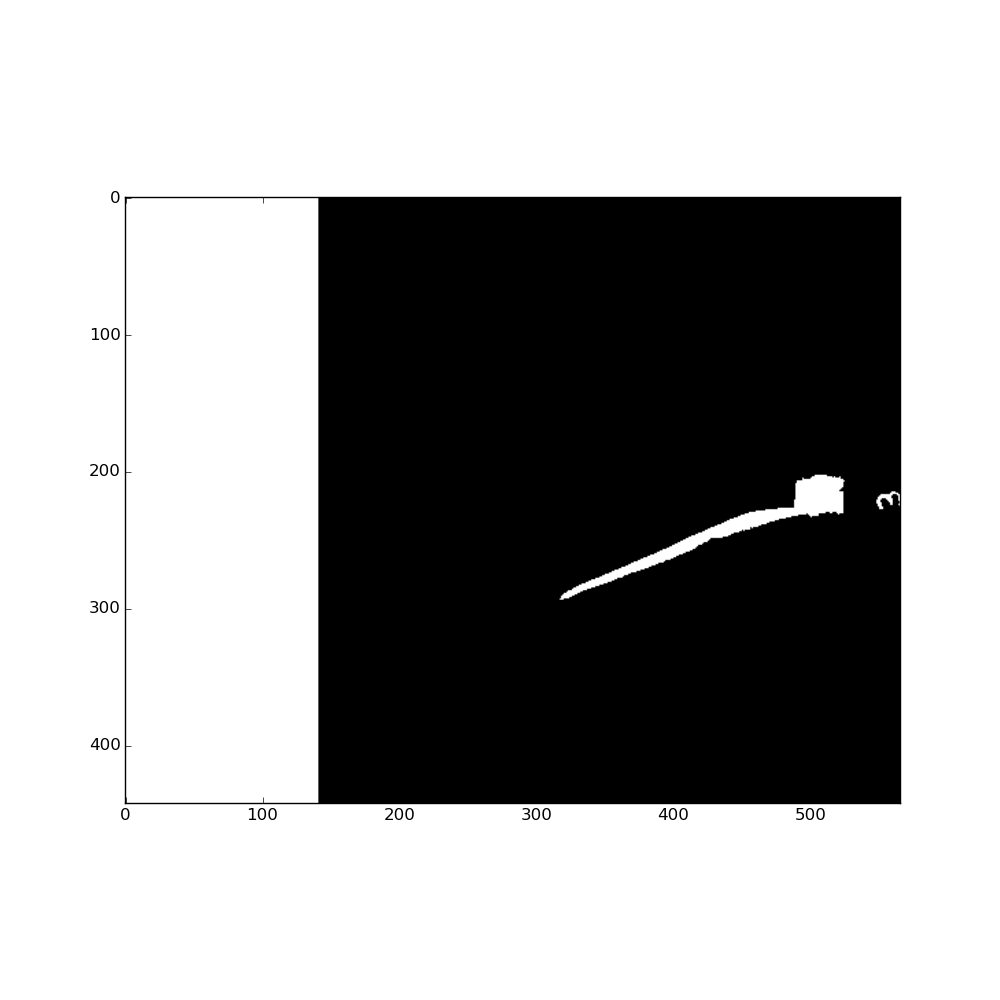
\includegraphics[width=0.37\textwidth]{resultados/Coral_3_S3_coral_otsu} % Include the image placeholder.png
\caption{Umbralización Otsu sobre la sección inferior de la imagen}
\label{fg:coral_otsu}
\end{center}
\end{figure}
\FloatBarrier


\begin{figure}[ht]
\begin{center}
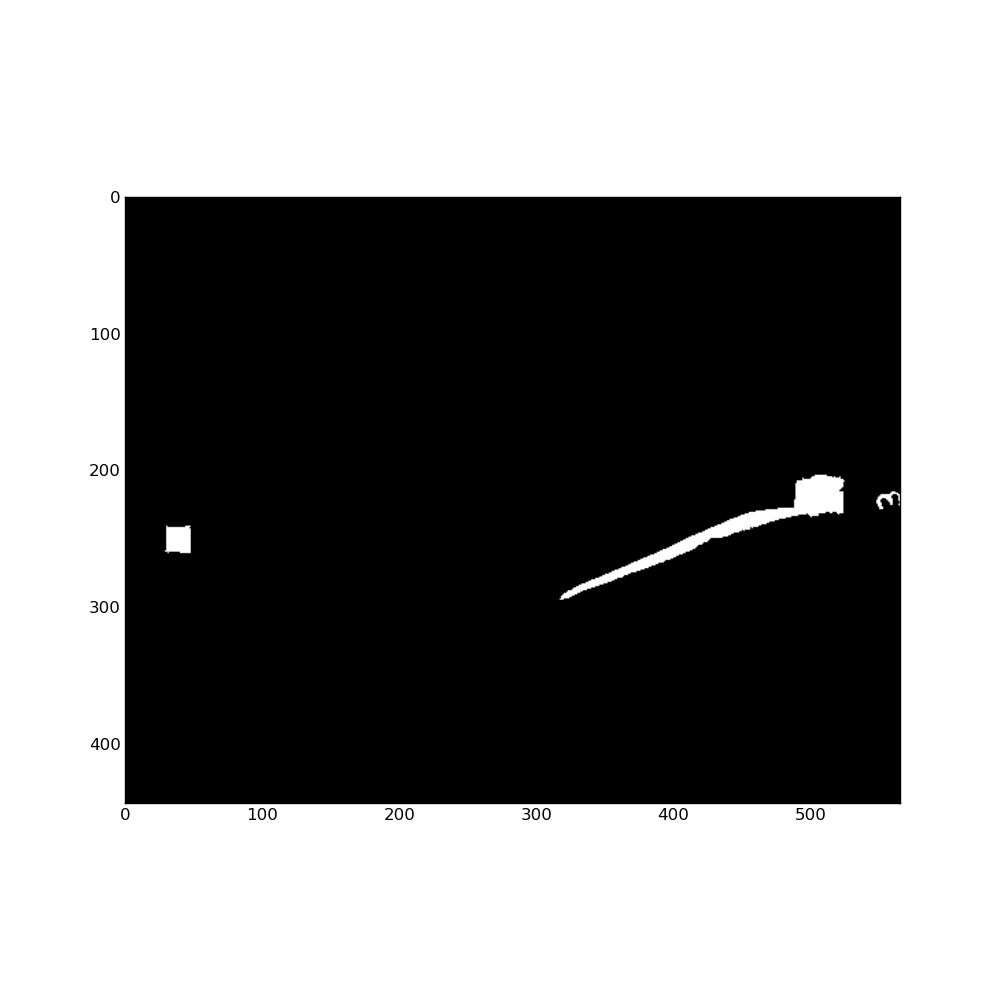
\includegraphics[width=0.37\textwidth]{resultados/Coral_3_S3_thresholded} % Include the image placeholder.png
\caption{Imagen Umbralizada}
\label{fg:umbral}
\end{center}
\end{figure}
\FloatBarrier

\begin{itemize}
    \item Componentes conectados
\end{itemize}

\begin{par}
Una vez obtenida la imagen umbralizada de manera correcta, el siguente paso trata de eliminar los objetos que no son de interes, es
decir en eliminar los objetos que no son ni el coral, ni el cuadrado de escala.\\
Para ello realizamos un análisis de reconocimiento de regiones por conectividad. Este análisis se basa en el concepto de conectividad.
Existen varias definiciones de conectividad. En la figura \ref{fg:connect} se expone el concepto de la 4-conectividad. Están conectados
a C los elementos 1 y no los elementos 0. C tiene 4 vecinos que están conectados. La 8-conectividad es intuitiva. Los elementos 0
en diagonal son ahora considerados como conectados a C igualmente. C tiene entonces 8 vecinos.\\
Se busca entonces en la imagen los diferentes componentes conectados y a cada uno se le asigna un nivel de gris distinto para diferenciarlos
los unos de los otros. Este análisis se realiza de manera independiente en la seccion superior de la imagen (cuadrado) y en la parte 
inferior (coral). Tanto el cuadrado como el coral son los componentes de área más grande en sus secciones independientes. Se puede entonces
eliminar respectivamente en la sección superior los componentes de área menor al área del cuadrado y eliminar en la parte inferior
los componentes de área menor al área del coral. Ya teniendo el componente del coral y del cuadrado a mano independientemente se realiza un proceso de dilatación y erosión para rellenar huecos pequeños que tengan estos dos objetos sin dañar su forma total.
\end{par}

\begin{figure}[ht]
\begin{center}
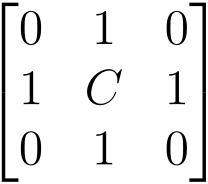
\includegraphics[width=0.10\textwidth]{resultados/connect} % Include the image placeholder.png
\caption{Ilustración del concepto de 4-conectividad}
\label{fg:connect}
\end{center}
\end{figure}
\FloatBarrier

\begin{itemize}
    \item Proceso de desarrollo
\end{itemize}

\begin{par}
Con la finalidad de establecer un mecanismo ágil de desarrollo de
software se hizo uso de una serie de herramientas para facilitar dicho
proceso. En primer lugar, se empleó un sistema de control de versiones en
línea con el propósito de implementar un sistema de administración del
código desarrollado. Adicionalmente, se utilizó un repositorio público
(GitHub) con la finalidad de que la comunidad interesada pueda consultar
los archivos fuentes del producto y realizar modificaciones, adiciones y
consultas. El repositorio mencionado puede ser consultado en el siguiente
vínculo: \url{https://github.com/sercharpak/Image_Analisis/tree/master/P
royecto}. Adicionalmente, se hizo uso de dos Notebooks de Python. Esta
herramienta permite realizar un proceso de desarrollo más interactivo en
el cual se puede combinar la ejecución de código con elementos de
gráficos. En particular, gracias al uso de Notebooks, fue posible
realizar ejecuciones parciales del código implementado y observar
resultados inmediatos en gráficas dispuestas en secciones intermedias. De
esta manera se facilitó el proceso de depuración e identificación de
errores.
\end{par}

\section{Resultados}

\begin{par}
Al finalizar el proceso se obtienen, de un lado, las imágenes con
únicamente el cuadrado de escala y el coral segmentado y por otro lado,
dos archivos de texto plano. Uno de los archivos contiene el área del
coral, en $cm^2$, y otro archivo contiene los datos de los pasos
intermedios realizados en el proceso. En las figura \ref{fg:final_1} y
\ref{fg:final_2} se pueden observar ejemplos de estas imágenes.
Únicamente contienen el cuadrado de escala y el coral umbralizado,
siempre se guardan en el caso se desea hacer un uso posterior de esta
información.
\end{par}

\begin{figure}[ht]
\begin{center}
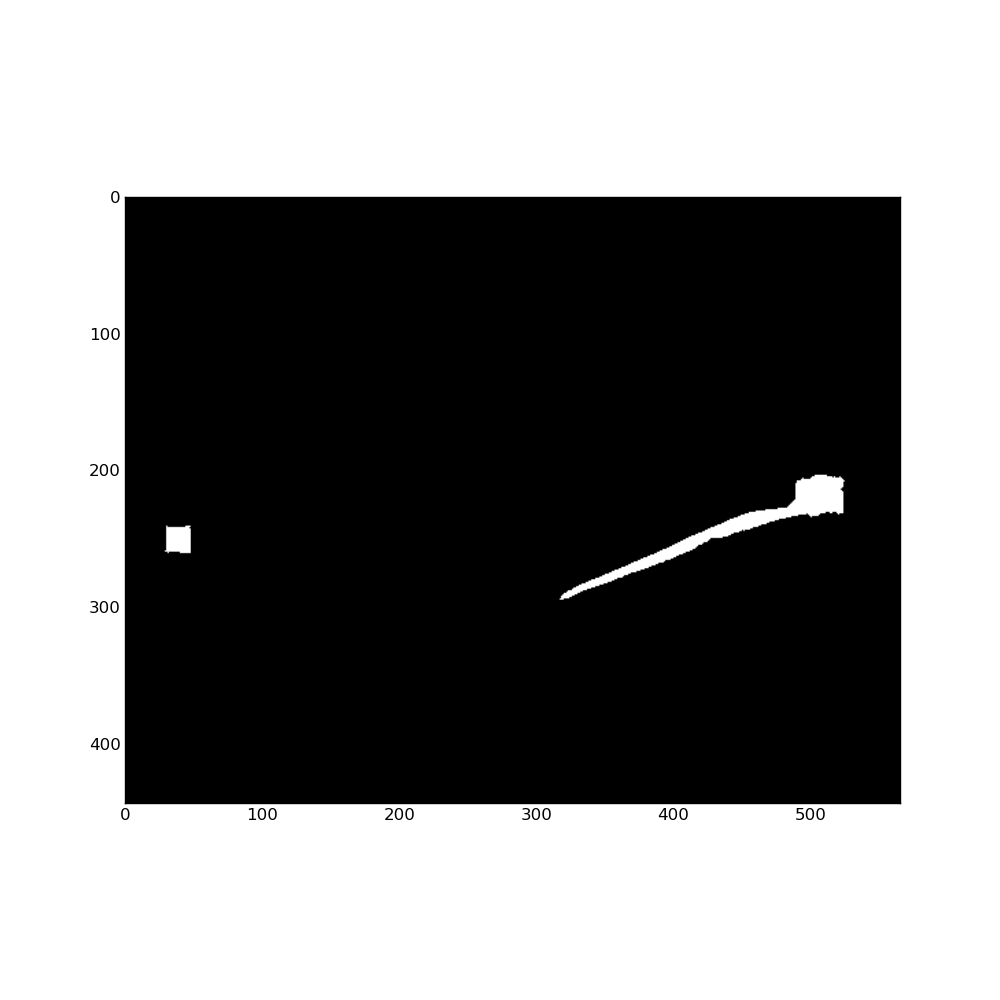
\includegraphics[width=0.40\textwidth]{resultados/Coral_3_S3_final_image} % Include the image placeholder.png
\caption{Ejemplo de imagen al finalizar el proceso}
\label{fg:final_1}
\end{center}
\end{figure}
\FloatBarrier

\begin{figure}[ht]
\begin{center}
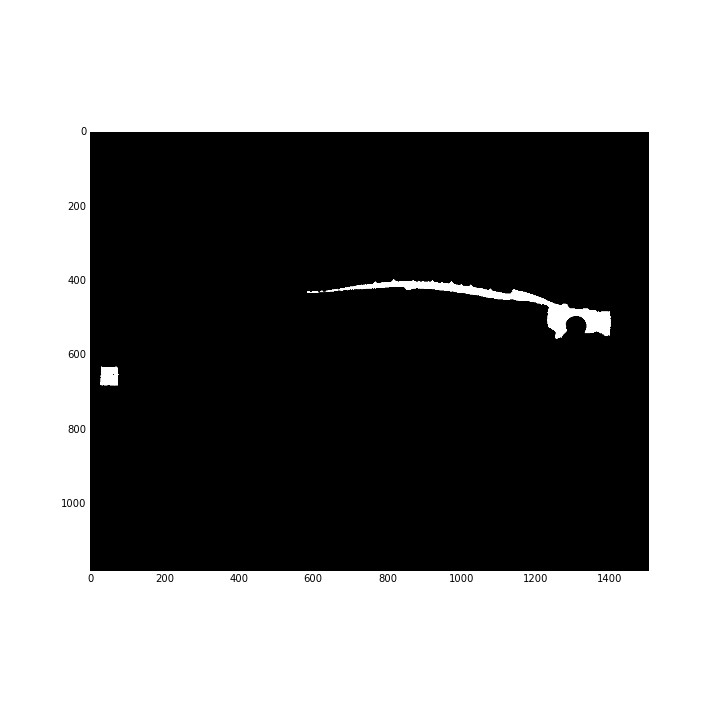
\includegraphics[width=0.40\textwidth]{resultados/Coral4_2_S2_final} % Include the image placeholder.png
\caption{Ejemplo de imagen al finalizar el proceso}
\label{fg:final_2}
\end{center}
\end{figure}
\FloatBarrier

\begin{par}
El otro resultado que obtenemos del proceso es el área en $cm^2$ del
coral. Para el análisis de una carpeta completa se obtiene un archivo de
texto con dos columnas, el nombre de la imagen, y su respectiva área. Un
ejemplo de esta tabla se puede observar en la tabla \ref{tab:results}
para una carpeta con 5 imágenes JPG.
\end{par}

\begin{table}[ht]
    \centering
    \begin{tabular}{|c|c|}
        Nombre Imagen & Área [ $ cm^2 $ ] \\
        Coral6\_S3   &  7.0 \\
        Coral\_3\_S3  &  7.0 \\
        Coral4\_S3   &  8.0 \\
        Coral4\_2\_S3 &  9.0 \\
        IMG\_6780    &  10.0 
    \end{tabular}
    \caption{Ejemplos de áreas calculadas al analizar una carpeta.}
    \label{tab:results}
\end{table}
\FloatBarrier

\begin{par}
El hecho que las áreas sean enteras en la tabla \ref{tab:results} es en
parte debido al número discreto de pixeles de las regiones encontradas.
Las áreas calculadas no necesariamente siempre serán números enteros. \\
\end{par}

\begin{par}
Con asesoría del grupo Biommar, se tuvo acceso a datos reales de
estas áreas. Sin embargo, debido a limitaciones de uso del software
actual Fiji con estas imágenes en partícular, se decidió que no eran
suficiente para validar nuestros resultados. Sin embargo se realizó el
proceso y se encontró que nuestros resultados tienen una discrepancia
debida a la base oscura en donde se encuentra atado el coral. Al
discutirlos con los expertos de Biommar, se decidió que tener el área de
dicha base era de gran interés también. A futuro se espera tener datos
por parte del experto para comparar de una manera cuantitativa los
resultados de este trabajo.
\end{par}

\begin{par}
Para detectar crecimiento coralino, se recomienda almacenar en la misma
carpeta las imágenes capturadas para un mismo coral en diferentes
instantes. Así, se podrá observar al analizar una sola vez la carpeta, el
crecimiento de área del coral.
\end{par}

\section{Conclusiones}
\begin{par}
En el presente proyecto se logró implementar un producto de software para
el análisis de imágenes de corales. En particular, se realiza la
determinación del crecimiento de estos organismos a través de una serie
de imágenes que son procesadas con técnicas especializadas.
Específicamente, se propuso un método basado en operaciones de
umbralización e identificación de componentes conexos para la
identificación del área del coral y de una referencia para definir las
mediciones en unidades reales. Adicionalmente, se realizan operaciones de
procesamiento adicionales como la erosión y el truncamiento de las
imágenes con el objetivo de reducir el ruido y, de esta manera, obtener
mediciones más precisas. El software desarrollado también está dispuesto
para realizar el cálculo directo del crecimiento o diferencia en área,
facilitando así el proceso de estudio para el grupo de investigación
Biommar.\\
\end{par}
\begin{par}
Al realizar un análisis sobre los resultados obtenidos se puede concluir
que se desarrolló un producto funcional que corresponde a los objetivos
propuestos. En particular, permite calcular el crecimiento coralino
tomando una serie de imágenes como parámetro de entrada. Al evaluar el
desempeño del producto con casos de prueba se obtuvieron mediciones
aceptables que efectivamente corresponden, aproximadamente, a los valores
obtenidos mediante el proceso manual. Sin embargo, las pruebas también
permitieron evidenciar las limitaciones del método propuesto.
Principalmente, se resalta el hecho de que el algoritmo está supeditado
directamente a los niveles de contraste en las fotografías tomadas. Esto
conlleva a que el producto tenga un alto nivel de dependencia respecto a
la toma de la fotografía en términos de iluminación y orientación. No
obstante, también cabe resaltar que el método de desarrollo de software y
la disposición del código fuente permiten realizar modificaciones con
relativa facilidad, de esta forma es posible ajustar los parámetros de
operación.\\
\end{par}
\begin{par}
Como posibles trabajos futuros sobre el producto desarrollado, se pueden incluir una serie de técnicas de procesamiento de imágenes para que el resultado no tenga un alto nivel de dependencia sobre la toma de las imágenes. En este caso, se podría pensar en incluir operaciones que consideren información adicional obtenida en la imagen, como datos estadísticos o características locales. Otro componente complementario que resultaría de gran utilidad para el grupo de investigación Biommar sería la determinación de la longitud del coral entendida como la medida del segmento central dispuesto entre los extremos del organismo
\end{par}


\section{Agradecimientos}
\begin{par}
Presentamos nuestros más sinceros agradecimientos a los integrantes del grupo Biommar por su disposición y por proveernos de las imágenes de prueba requeridas para las pruebas del producto implementado. Particularmente agradecemos a Susana Simancas y Nancy Estefanía Ruiz Uribe por la disposición,  colaboración y tiempo que brindaron a este trabajo a lo largo de todo el proyecto. También agradecemos a Marcela Hernández por su constante asesoría a lo largo del desarrollo del producto.
\end{par}


%\section{Conclusion}
%\blindtext

%\appendices
%\section{Proof of the First Zonklar Equation}
%Some text for the appendix.

% use section* for acknowledgement
%\section*{Acknowledgment}


%The authors would like to thank...

%\ifCLASSOPTIONcaptionsoff
%  \newpage
%\fi

\bibliographystyle{IEEEtran}
\bibliography{references}

%\begin{IEEEbiography}[{
\includegraphics[width=1in,height=1.25in,clip,keepaspectratio]{picture}}]{John Doe}
%\blindtext
%\end{IEEEbiography}

\end{document}


